% This is both incomplete & not self-contained.
% The plots with better resolution are yet to be added.
% Relevant Indico: 
% - Real Backgrounds: https://indico.cern.ch/event/1200632/contributions/5048435/attachments/2513037/4319901/gnn-application-on-background-mc-samples.pdf
% - Fake Backgrounds: 
%    - More up-to-date: https://indico.cern.ch/event/1309827/contributions/5509564/attachments/2688607/4665119/fake-backgrounds-in-rkstar-updated.pdf
%    - More detailed: https://indico.cern.ch/event/1307390/contributions/5499421/attachments/2684051/4656482/background-for-RKStar-v2.pdf

% %%% Chapter Title %%%
% %%% ------------- %%%
% \chapter{A Study of ``Structured'' Backgrounds}
% \label{chap:a-study-in-fake}

%%% Introduction %%%
%%% ------------ %%%
\subsection{Introduction}
\label{subsec:back-intro}

Not all backgrounds are created equal; some are peskier than others. % 
In particular, any background that can form a \emph{distinctive structure} in its distribution in the discriminating variable, i.e., the variable in whose distribution the final fit is performed, needs to be studied in its own right. %
\\\\
As such, we expect the most dominant sources of background to be combinatorial and partially reconstructed decays. %
Such sources of background are not expected to form any distinctive structure in their distribution of $m(B)$ which is the discriminating variable in this analysis. %   
Outside of the combinatorial and the partially reconstructed sources of background, which are essentially monotonic (i.e. non-structured), there exist other sources of background that can be genuinely distinctively structured in the signal region of $m(B)$. %
One can identify two such sources of background:
\begin{enumerate}
    \item \textbf{Real Backgrounds}: The decays of particles whose masses lie in the fit-region of $m(B)$ and whose decay structures (number of final-state particles, their vertexing, etc.) are similar to that of the signal decay. 
    \item \textbf{Fake Backgrounds}: The decays of particles whose masses lie in the fit-region of $m(B)$ and whose decay structures can be made to look similar to that of the signal decay if the final-state particles are misidentified.
\end{enumerate} 
One important point to notice is that despite such sources of backgrounds being significantly subdominant compared to the combinatorial and partially reconstructed decays, they matter just as much (in terms of the analysis strategy) so long as their yield is comparable to the signal yield, as it was well demonstrated in the LHCb measurement from December 2022~\cite{LHCbDec2022}. % 
Given that we are measuring a rare decay with a branching fraction $\mathcal{O}(10^{-6})$, we are precisely in the situation, where we cannot neglect even such subdominant sources of background. % 
\\\\
Our goal in the study of these backgrounds is to understand two aspects:
\begin{enumerate}
    \item Do they actually form a distinctive (non-monotonic) structure in the distribution of $m(B)$? 
    \item If they do, how do we deal with them?
    \begin{itemize}
        \item Can some targeted cuts be applied to reject them?
        \item If not, how should these be modeled in the final fit?
    \end{itemize}
\end{enumerate}
The study of such backgrounds with the goals outlined above constitutes the majority of the ongoing work in the analysis. %
In the following, I will outline the strategy that we are following to study such backgrounds.

%%% The Real Backgrounds %%%
%%% -------------------- %%%
\subsection{The Real Backgrounds}
\label{subsec:the-real-backgrounds}

The real backgrounds in this analysis are expected to arise from the decays of $B$-hadrons other than the signal decay. %
Since such decays are expected to look very similar to signal decay, we cannot easily reject them using either heuristic cuts or multivariate techniques without losing much of our signal efficiency. % 
However, specific sources of real backgrounds can be targeted by designing specific heuristic cuts, for example, $B_s^0 \to \phi(1020)(\to K^+K^-) \ell^+\ell^-$ can be targeted by rejecting events with an invariant mass of the $K^+K^-$ pair that is very close to the $\phi(1020)$ meson (this cut is already employed). %
The residual of the real backgrounds needs to be modeled in the final fit (for example, as in the $B^+$ case discussed earlier). %
We are working on both the design of the cuts to reject specific sources of real backgrounds as well as the modeling of the residual of the real backgrounds in the final fit. %
These backgrounds are expected to form a peaking structure under the signal $B-$mass, particularly in the high$-q^2$ bin as can be seen in Fig.~\ref{fig:peaking-real-background-mc}. %
Both of these efforts rely on the use of the MC simulation of the relevant backgrounds. %
In particular, the shape of the fit model of the residual of the real backgrounds is to be obtained from the MC simulation of the relevant backgrounds while the yield of the residual of the real backgrounds is to be tied to the yield of the signal in the resonant channel. %
\begin{figure}[!ht]
    \centering
    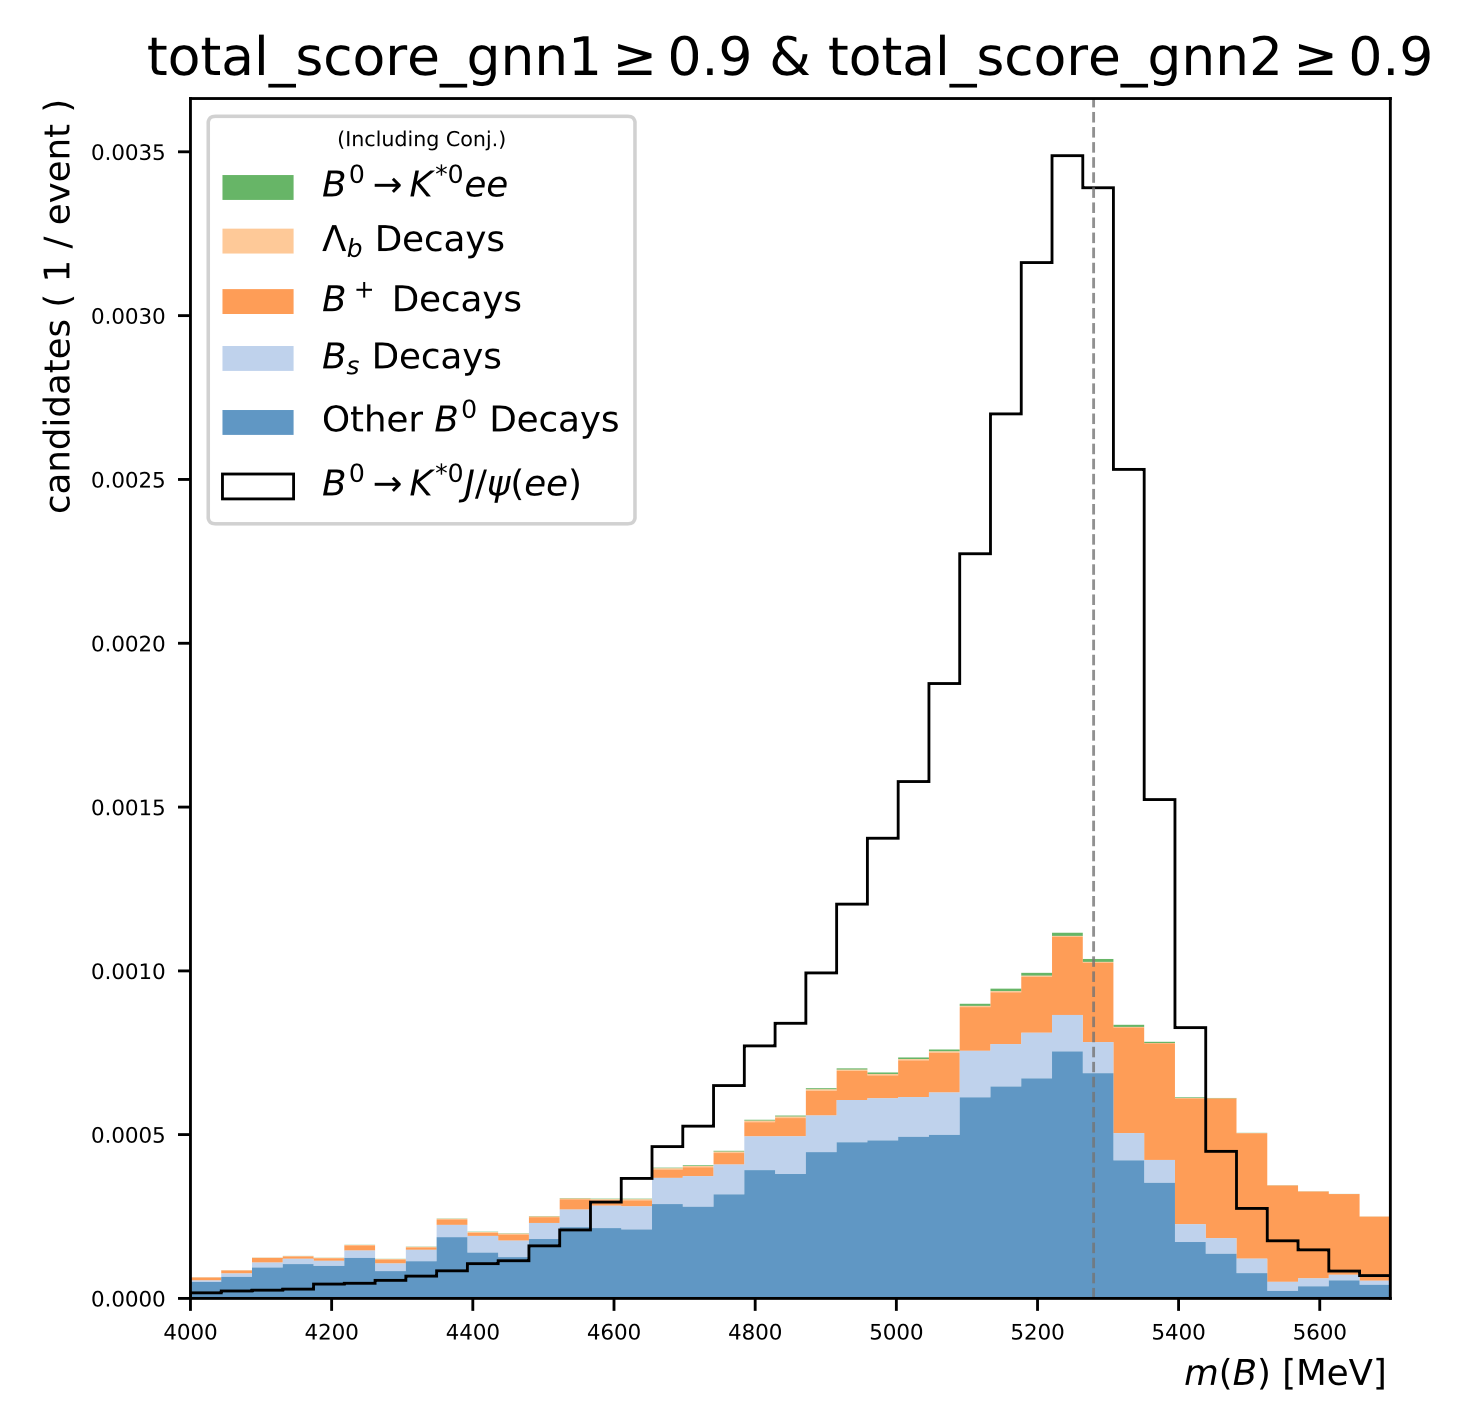
\includegraphics[width=0.48\textwidth]{figures/stacked-b-mass-q2high.png}
    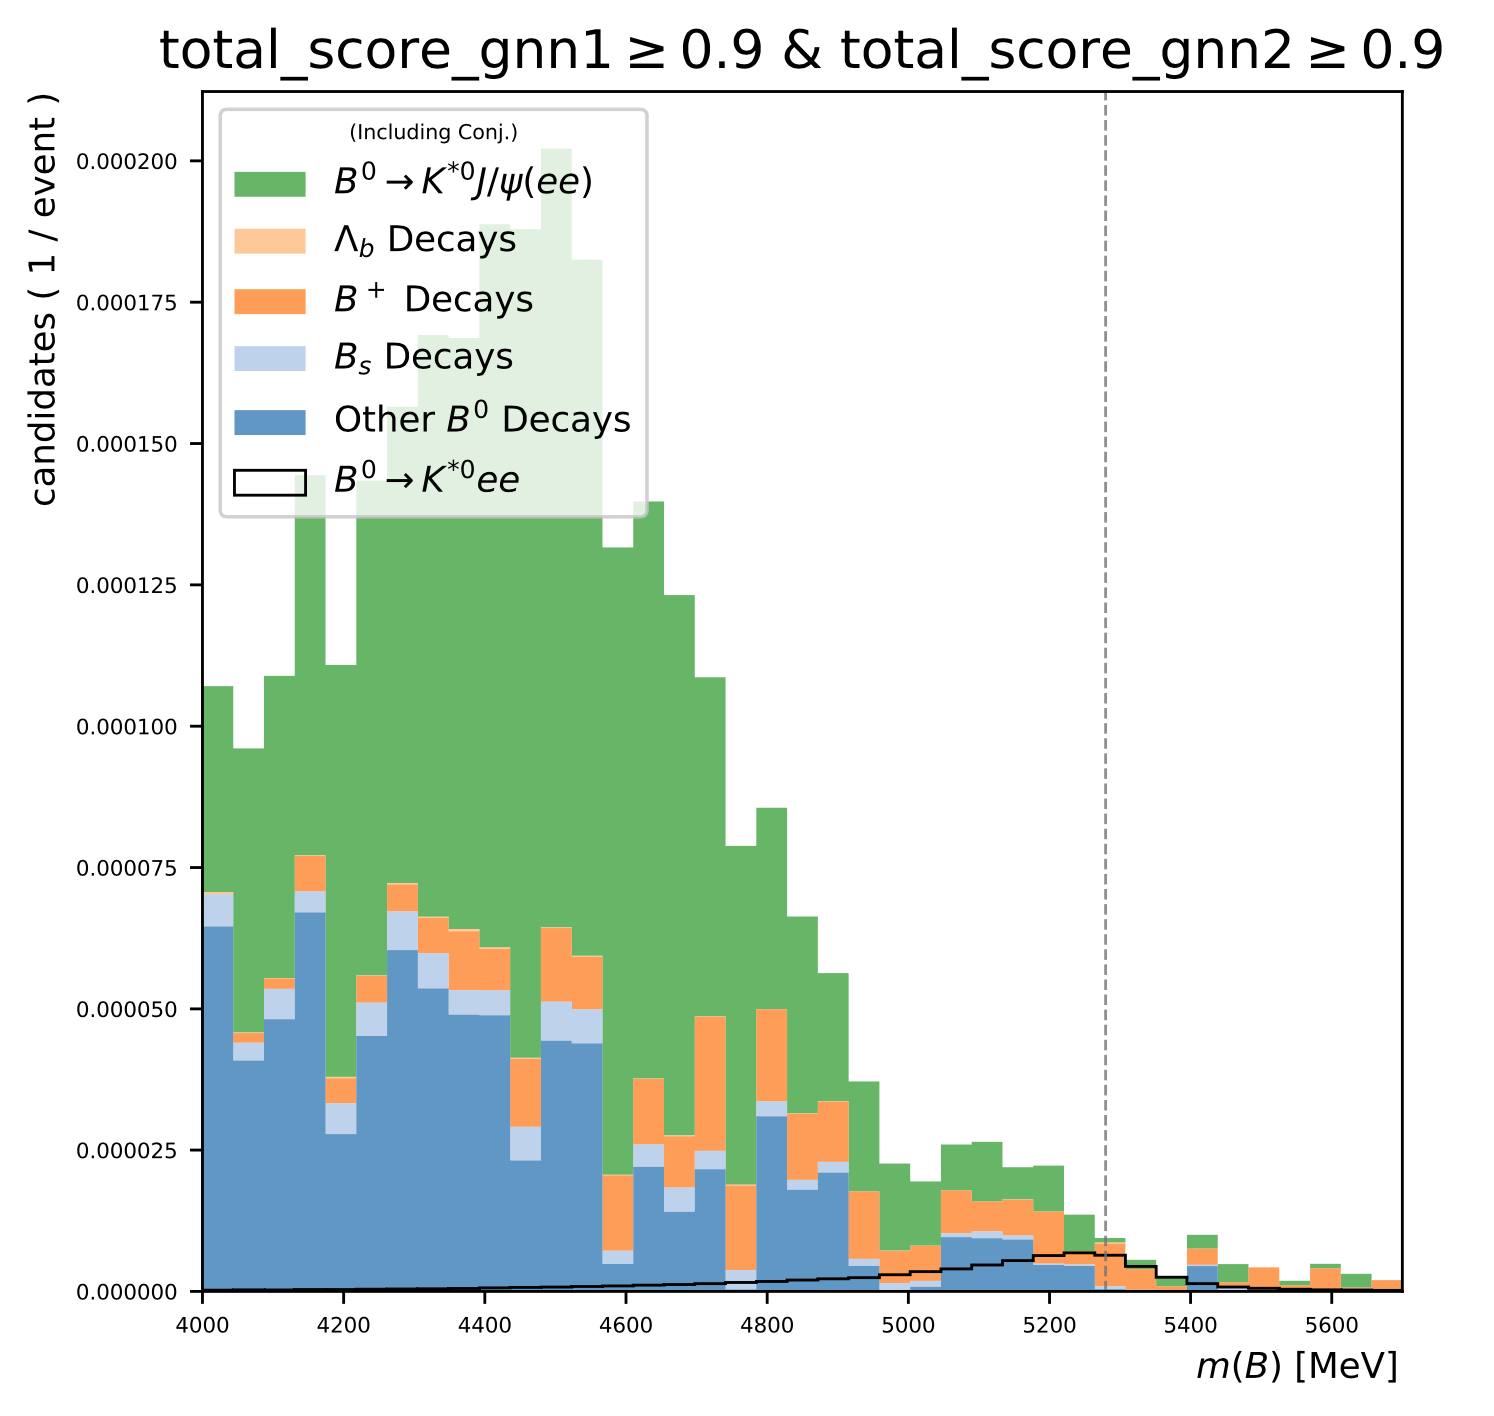
\includegraphics[width=0.48\textwidth]{figures/stacked-b-mass-q2low.png}
    \caption{Comparison of the signal to the cumulative contribution from major sources of real background after stringent cuts on the GNN scores: signal being $B_d^0\to K^{\ast 0}(K^+\pi^-)J/\psi(e^+e^-)$ in the high$-q^2$ bin (left), $B_d^0\to K^{\ast 0}(K^+\pi^-)e^+e^-$ in the low$-q^2$ bin (right). All distributions are normalized to the same (albeit arbitrary) luminosity so as to correctly represent their relative yields.}
    \label{fig:peaking-real-background-mc}
\end{figure}
\\\\
We are currently running a large MC campaign to complete the list of real backgrounds for completeness where the list is being compiled using the~{\texttt{decaylanguage}} package\footnote{\href{https://github.com/scikit-hep/decaylanguage}{\texttt{\textcolor{olive}{https://github.com/scikit-hep/decaylanguage}}}}. %
This is relevant for both the electron and the muon channels of the measurement. %

%%% The Fake Backgrounds %%%
%%% -------------------- %%%
\subsection{The Fake Backgrounds}
\label{subsec:the-fake-backgrounds}

The $R(X)$ measurement is particularly sensitive to the estimation of the fake backgrounds in the electron channel. %
For example, as mentioned earlier, the source of tension with the SM in the pre-2022 LHCb measurements of $R(K)$ and $R(K^{\ast})$ has been attributed to the missing estimation of the background arising from hadrons faking electrons. % 
Also in this analysis, the fake backgrounds are expected to arise from the misidentification of final-state hadrons (mostly pions, kaons, and protons) as electrons or muons; as well as, to a lesser extent, from the misidentification of final-state photons as electrons via the conversion of the photon into an $e^+e^-$ pair in the detector material. %
\\\\
We are studying three different methods to model the fake backgrounds in the final fit: the matrix method, the reverse-region method, and the MC-driven method. % 
The first two of these methods are data-driven methods while the third one simply relies on the MC simulation of the relevant backgrounds. %
It is usually considered unreliable to purely rely on the MC simulation of the fake backgrounds because the MC simulation is not expected to model the misidentification rates very well. %
However, the MC-driven method is still useful as a cross-check on the other two methods. %
Concerning the data-driven method, the bottleneck is the availability of a fake-enriched region of the data. %
This is a control region of the data, where we expect the hadrons to be the dominant source of reconstructed leptons. %
\\\\
In the electron channel, the methods that are traditionally used to define such a region are not applicable: we cannot use the isolation variables to define the fake-enriched region because both the signal and the fake backgrounds are expected to be non-isolated; we cannot easily reverse the particle identification cuts because our electrons are already at the loosest possible working point of the particle identification. %
Thus, we are exploring the utilization of low-level information associated with the tracks of the reconstructed leptons to define a fake-enriched region of the data. %
Another ongoing effort is the study of decay modes that are expected to be particularly important in the estimation of fake backgrounds. %
It is crucial to prepare a representative sample of the fake backgrounds in the MC simulation. %
Such a sample is also necessary to validate the extraction of the fake-enriched region in the data-driven methods. %
We are currently running a large MC campaign to complete the list of fake backgrounds where the list is being compiled using the~{\texttt{decaylanguage}} package mentioned earlier. %
This is relevant mainly for the electron channel of the measurement. %
\\\\
The estimation of the fake muon background will follow with more traditional methods since the muons are not at the loosest identification levels. %
In addition, the impact of fake muons is usually much smaller compared to the one from fake electrons. %
\\\\
